\section{更换网络：强预训练下 CORAL 还提供什么？}
\label{sec:backbone}

\subsection{探索动机与实验设计}

前两部分表明，继续增加约束或调节强度并没有形成一致收益。由此转向表示本身：使用更强的预训练主干之后，目标域表现是否改善，CORAL 是否仍能提供可辨认的额外作用？本阶段将 AlexNet 换为 ImageNet V2 预训练 ResNet-50，比较无 CORAL、logits、pooled、layer4 及两种含 logits 的联合设置。

logits 为 31 维输出；pooled 为 2,048 维全局空间均值；layer4 为末级残差相加及 ReLU 后的空间通道特征。layer4 仍将空间位置合并后估计通道协方差。固定 $\lambda=0.5$，多层取均值；SGD 主干学习率 0.001、分类头 0.01，momentum 与 weight decay 沿用前述设置。batch 调整为 32，每轮 24 次更新，输入使用 Resize(224) 和按域归一化。五个 CORAL 组使用第二部分的训练损失停止规则，未触发则运行 100 轮；无 CORAL 组运行至 100 轮。

\textbf{无 CORAL 对照采用相同的共享 BatchNorm。}每步按源域、目标域顺序前向，两域均更新 BN 统计量；评估时冻结。即使不使用适应损失，目标域输入也已影响模型。

\subsection{实验结果与停止信号}

表\ref{tab:resnet}与图\ref{fig:resnet}报告停止轮表现。无 CORAL 组第 100 轮为 80.00\%。pooled 与 layer4 单独对齐均跑满 100 轮，准确率为 80.38\% 与 79.87\%，同轮差值为 $+0.38\pp$ 与 $-0.13\pp$。这两种特征统计约束在当前协议下没有提供清晰的额外分类收益。

\begin{table}[H]
 \centering\small
 \caption{ResNet-50 V2 的 CORAL 比较。准确率单位为 \%。同轮对照取无 CORAL 组在对应停止轮的准确率，不统一减去其第 100 轮结果。}
 \label{tab:resnet}
 \begin{tabular}{lrrrr}
 \toprule
 配置 & 停止轮 & 准确率 & 同轮对照 & 差值（pp）\\
 \midrule
 \ResnetRows
 \bottomrule
 \end{tabular}
\end{table}

含 logits 的三个配置观察到正向同轮收益：logits 第 37 轮为 81.01\%，对照为 78.49\%；pooled+logits 第 42 轮为 80.25\%，对照为 78.11\%；layer4+logits 第 42 轮为 81.76\%，对照为 78.11\%。相应增益为 2.52、2.14、3.65 pp。这说明强预训练下 CORAL 的作用依赖对齐位置，且 CORAL 在这一预训练网络上的效果已经微乎其微。

\begin{figure}[H]
 \centering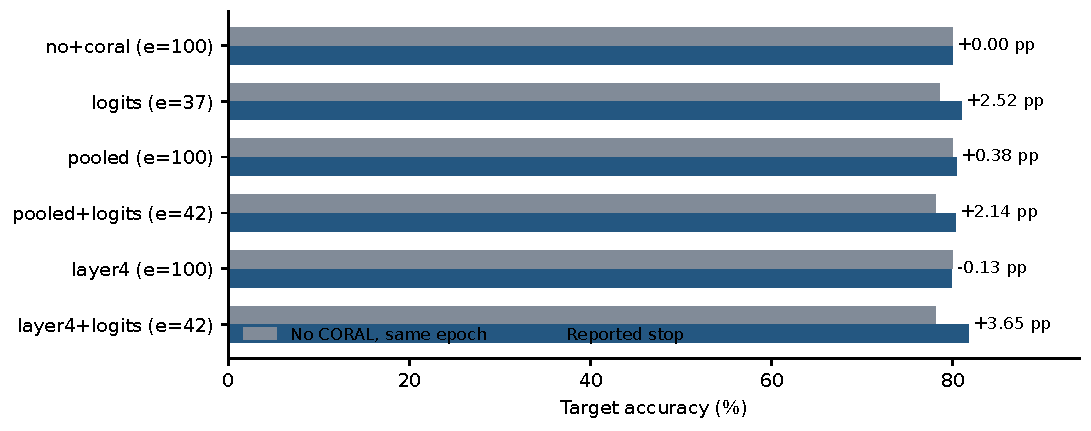
\includegraphics[width=\linewidth]{resnet_coral.pdf}
 \caption{ResNet CORAL 的停止轮及同轮对照。柱旁为同轮百分点差。无 CORAL 对照也利用目标图像更新 BN，全部横柱从零起绘制。}
 \label{fig:resnet}
\end{figure}

损失平衡与分类峰值也出现分离。三个含 logits 的组分别在第 37、42、42 轮停止，其目标准确率峰值却都出现在第 22 轮。相较之下，pooled 与 layer4 的最终加权 CORAL 项分别约为 CE 的 4.68\%、49.28\%，没有满足两项损失接近的停止条件。不同层的距离与梯度具有不同尺度，即使使用相同 $\lambda$，也不意味着相同的优化约束。

\subsection{阶段结论与反思}

更换网络后，无 CORAL 配置的目标准确率达到 80.00\%，实验表明预训练、微调和共享 BN 的组合能够形成较强的迁移参照。含 logits 的 CORAL 仍提供了可观察的同轮增益，而单独 pooled、layer4 没有形成同样的变化。考虑到此时 CORAL 带来的提升已经非常小了，我们转向另一个问题：全局二阶统计没有直接保留类别对应关系，能否通过选择更合适的对齐对象改善迁移？
